\subsection{Scénario Cockburn}
\textbf{Cas d'utilisation: }Rentrer

\textbf{Acteur primaire:} Le conducteur

\textbf{Pré-condition: } La voie est libre et ouvertre.
 
\textbf{Post-condition: } le systeme de paiement est opérationnel


\textbf{Scenario primaire: } \\
    \textbf{1.} La boucle repère le véhicule.\\
    \textbf{2.} La boucle envoi l’information à la borne.\\
    \textbf{3.} La borne détermine le type de véhicule. Le type est autorisé \\
    \textbf{4.} La borne afficher le montant.

\textbf{Variantes:}\\
    \textbf{1a.} La boucle ne repère pas le véhicule, l’utilisateur ne peut pas passer. Il doit appeler le technicien. Fin scénario.\\
    \textbf{3a.} L’opérateur repère un véhicule prioritaire en urgence. Il ouvre la barrière manuellement. Fin scénario \\
    \textbf{3b.} La borne détermine le type de véhicule. Le type n’est pas autorisé. Il appelle le technicien.\\
    \textbf{4a.} La borne n’affiche pas le montant, l’utilisateur ne peut pas payer il appelle le technicien.\\
\newpage    
\subsection{Diagramme d'activité}
\begin{figure}[!htb]
    \centering
    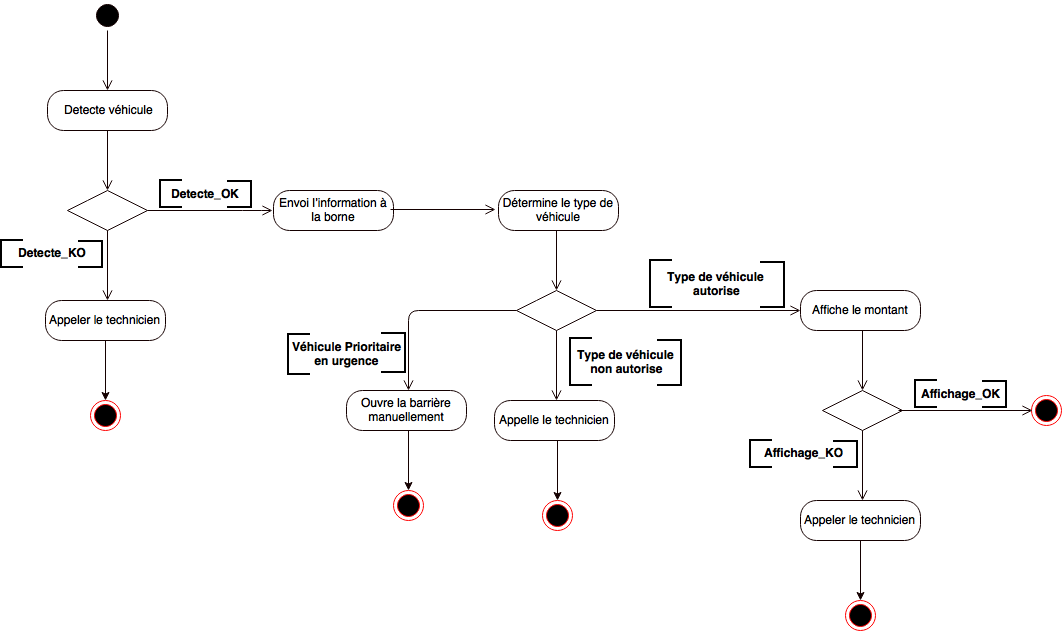
\includegraphics[scale=0.45, angle = 90]{02_Desenvolvimento/TD2/images/DARentrer.png}
    \caption{Diagramme d'activité - Rentrer}
    \label{fig:DARentrer}
\end{figure}
\newpage    
\subsection{Collaboration}
\begin{figure}[!htb]
    \centering
    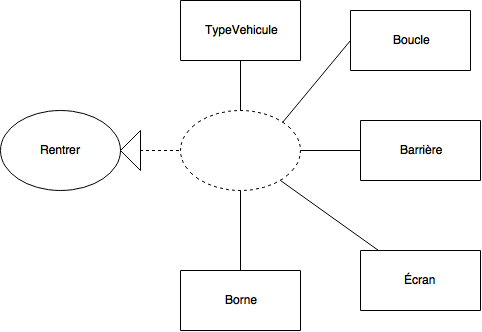
\includegraphics[scale=0.6]{02_Desenvolvimento/TD2/images/ColaRentrer.png}
    \caption{Collaboration - Rentrer}
    \label{fig:DARentrer}
\end{figure}